% ------------------------------------------------------------------------------
% Chapter 3
% ------------------------------------------------------------------------------
\chapter{Deciding Models and Model Building}
\label{cha:chapter 3}

\section{Model Selection}
\label{sec:chap3 section 1}

In this section, we describe the model selection procedures that are followed. It involved evaluating various architectures to identify the one that best captures the patterns in the data while avoiding overfitting. The process typically includes experimenting with different network depths, layer types, and hyperparameters. In this project, we tested several models to determine the most suitable architecture for our task.

\textbf{Model 1: Convolutional Neural Network (CNN)}
The first model tested was a Convolutional Neural Network (CNN) designed to extract spatial hierarchies from the input images. The model architecture includes multiple convolutional layers, each followed by a ReLU activation function, pooling layers, and dropout layers to prevent overfitting. This architecture leverages the spatial structure of the images, making it well-suited for image classification tasks such as pneumonia detection. The model architecture is given in appendix \ref{app:app-A section2}.

\textbf{Model 2: Enhanced CNN with Adam Optimizer}
The second model is an enhanced version of the initial CNN, which incorporates the Adam optimizer instead of RMSprop. This change was made to potentially improve the model's convergence and overall performance. The architecture remains similar but with fine-tuning of the optimizer parameters. The model architecture is given in appendix \ref{app:app-A section3}.

\textbf{Model 3:  simplified architecture with fewer layers and parameters for Target Variable Prediction}
This model uses two convolutional layers followed by max pooling, dropout, and a dense layer before the output. The results indicated more stable training and validation metrics compared to the previous models, suggesting better generalization. It should be noted that the model is trained for the \emph{Target} variable rather than the class labels. The model architecture is given in appendix \ref{app:app-A section4}.

\section{Model Building}
\label{sec:chap3 section 2}

Model 1 was trained on the pre-processed dataset using an 80:20 train-validation split. The training process involved monitoring both training and validation accuracy and loss to assess the model's performance and generalization capability. Figure \ref{fig:chap3 figure1} shows the training and validation accuracy and loss curves for Model 1.

\begin{figure}[H]
    \centering
    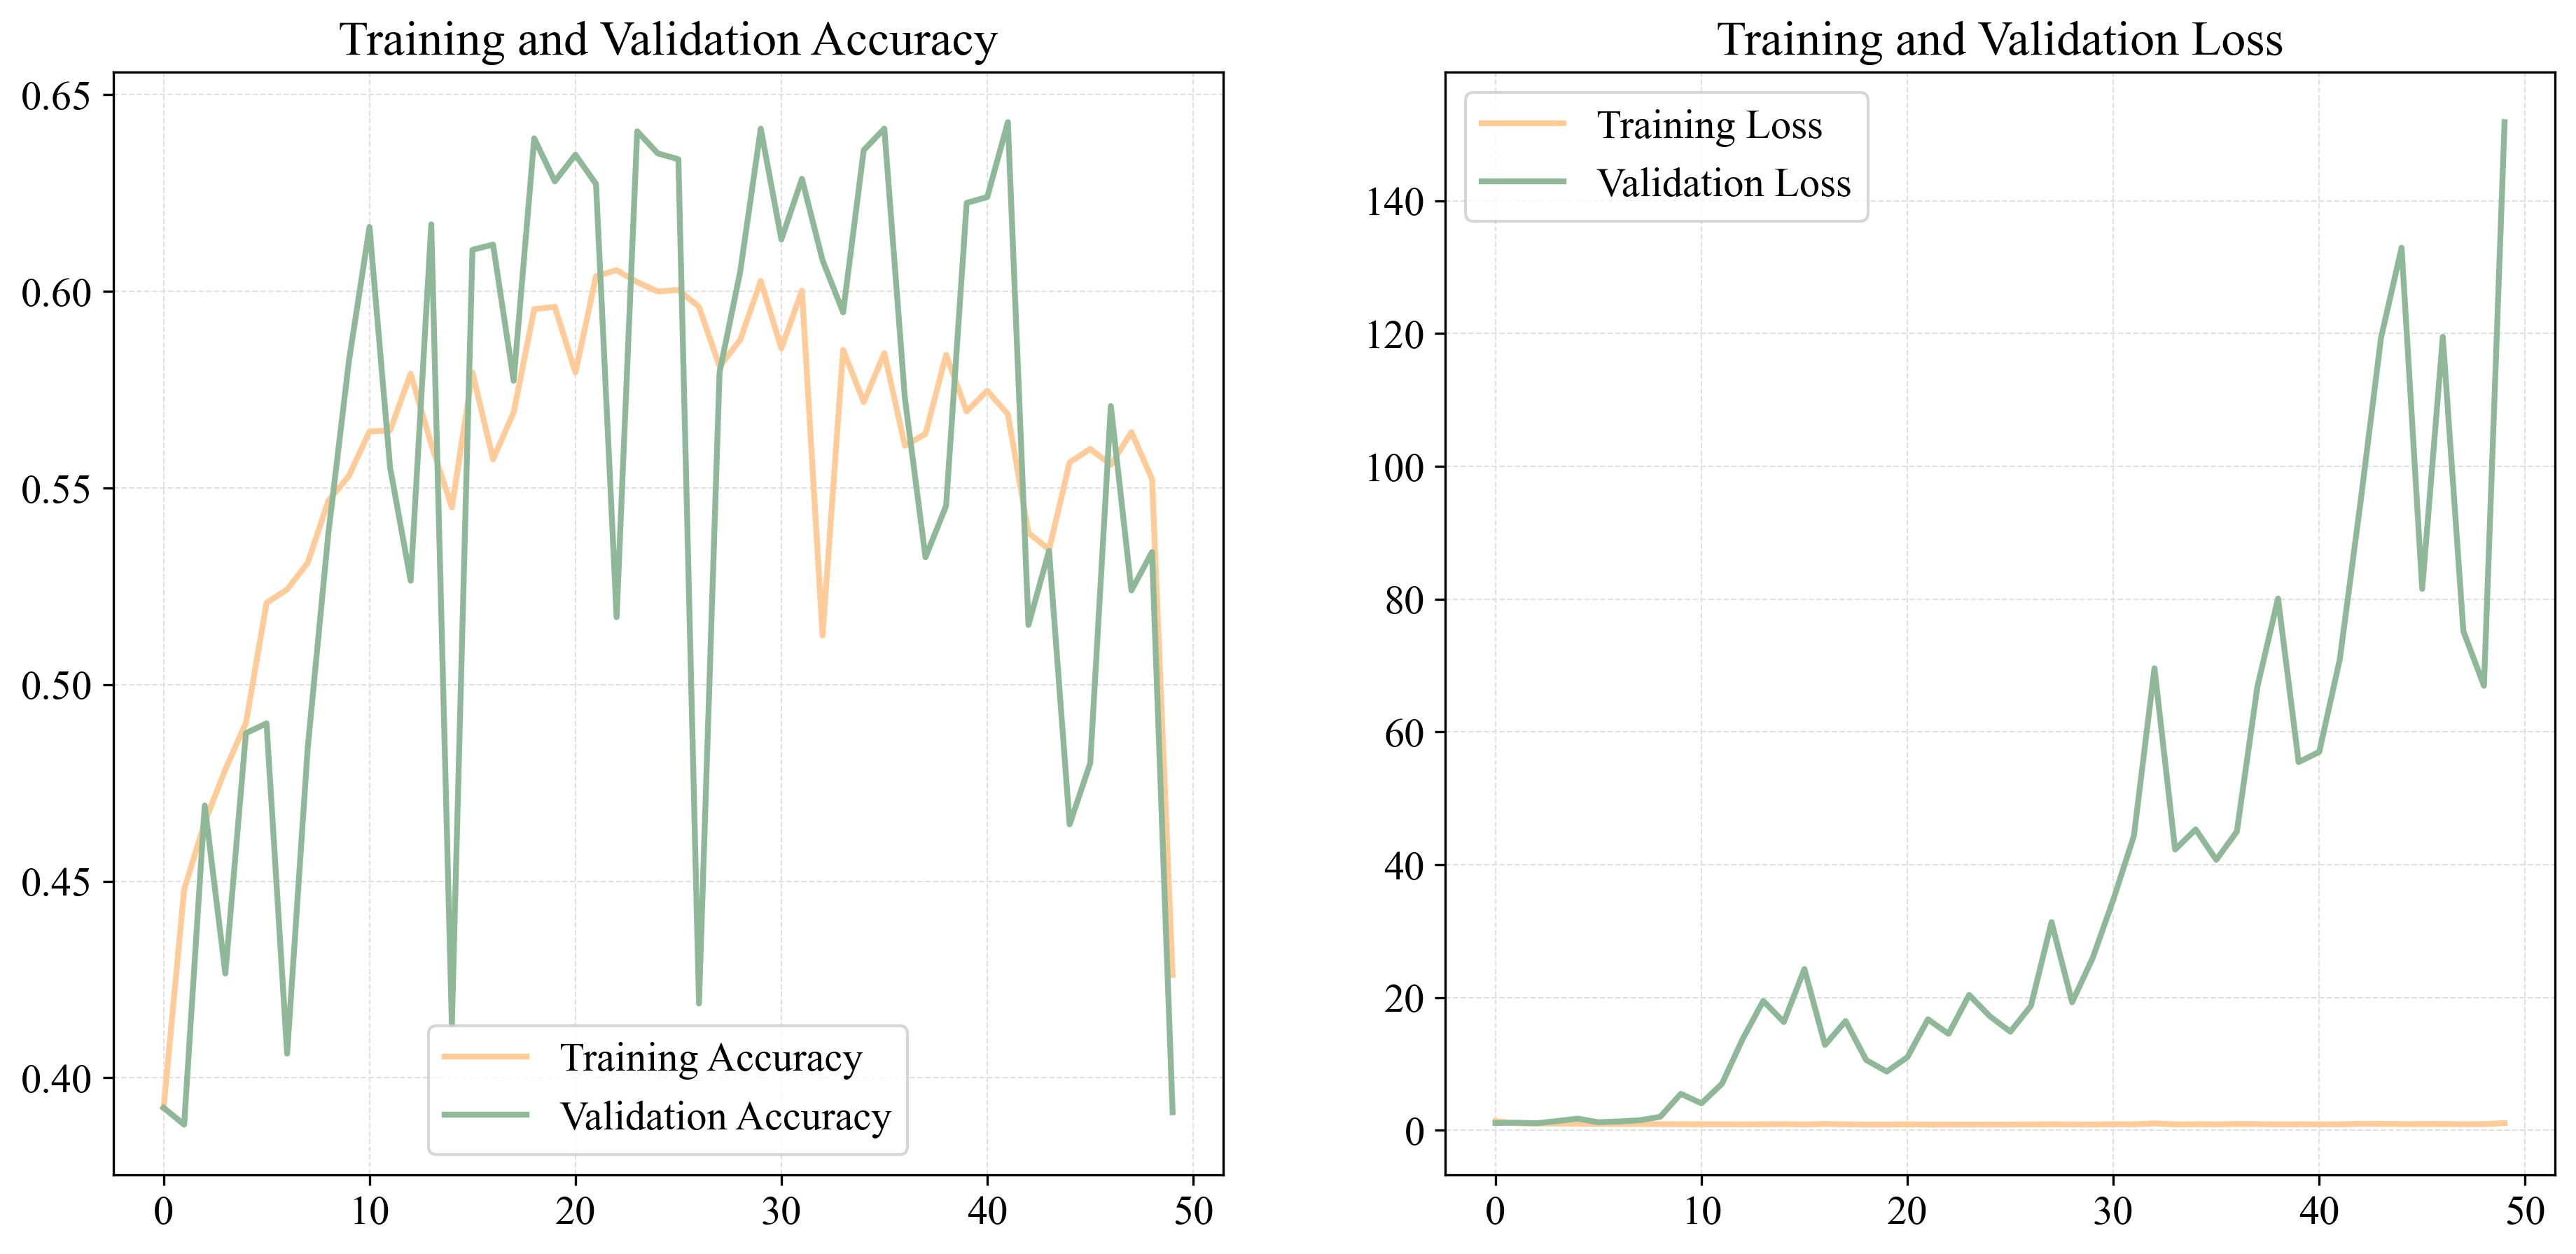
\includegraphics[width=0.8\textwidth]{figures/Figure29.png}
    \caption{Training and Validation Accuracy and Loss Curves for Model 1}
    \label{fig:chap3 figure1}
\end{figure}

\textbf{Key Observations:}
\begin{itemize}
    \item \textbf{Training Accuracy and Loss:} The training accuracy steadily improved over the epochs, indicating that the model was learning the patterns in the training data. The training loss decreased correspondingly.
    \item \textbf{Validation Accuracy and Loss:} The validation accuracy exhibited fluctuations but showed an overall increasing trend, suggesting that the model was able to generalize to some extent. However, the validation loss showed significant fluctuations, indicating potential overfitting.
\end{itemize}

Model 2 was trained on the pre-processed dataset using an 80:20 train-validation split. The training process involved monitoring both training and validation accuracy and loss to assess the model's performance and generalization capability. Figure \ref{fig:chap3 figure2} illustrates the training and validation accuracy and loss over 50 epochs.

\begin{figure}[H]
    \centering
    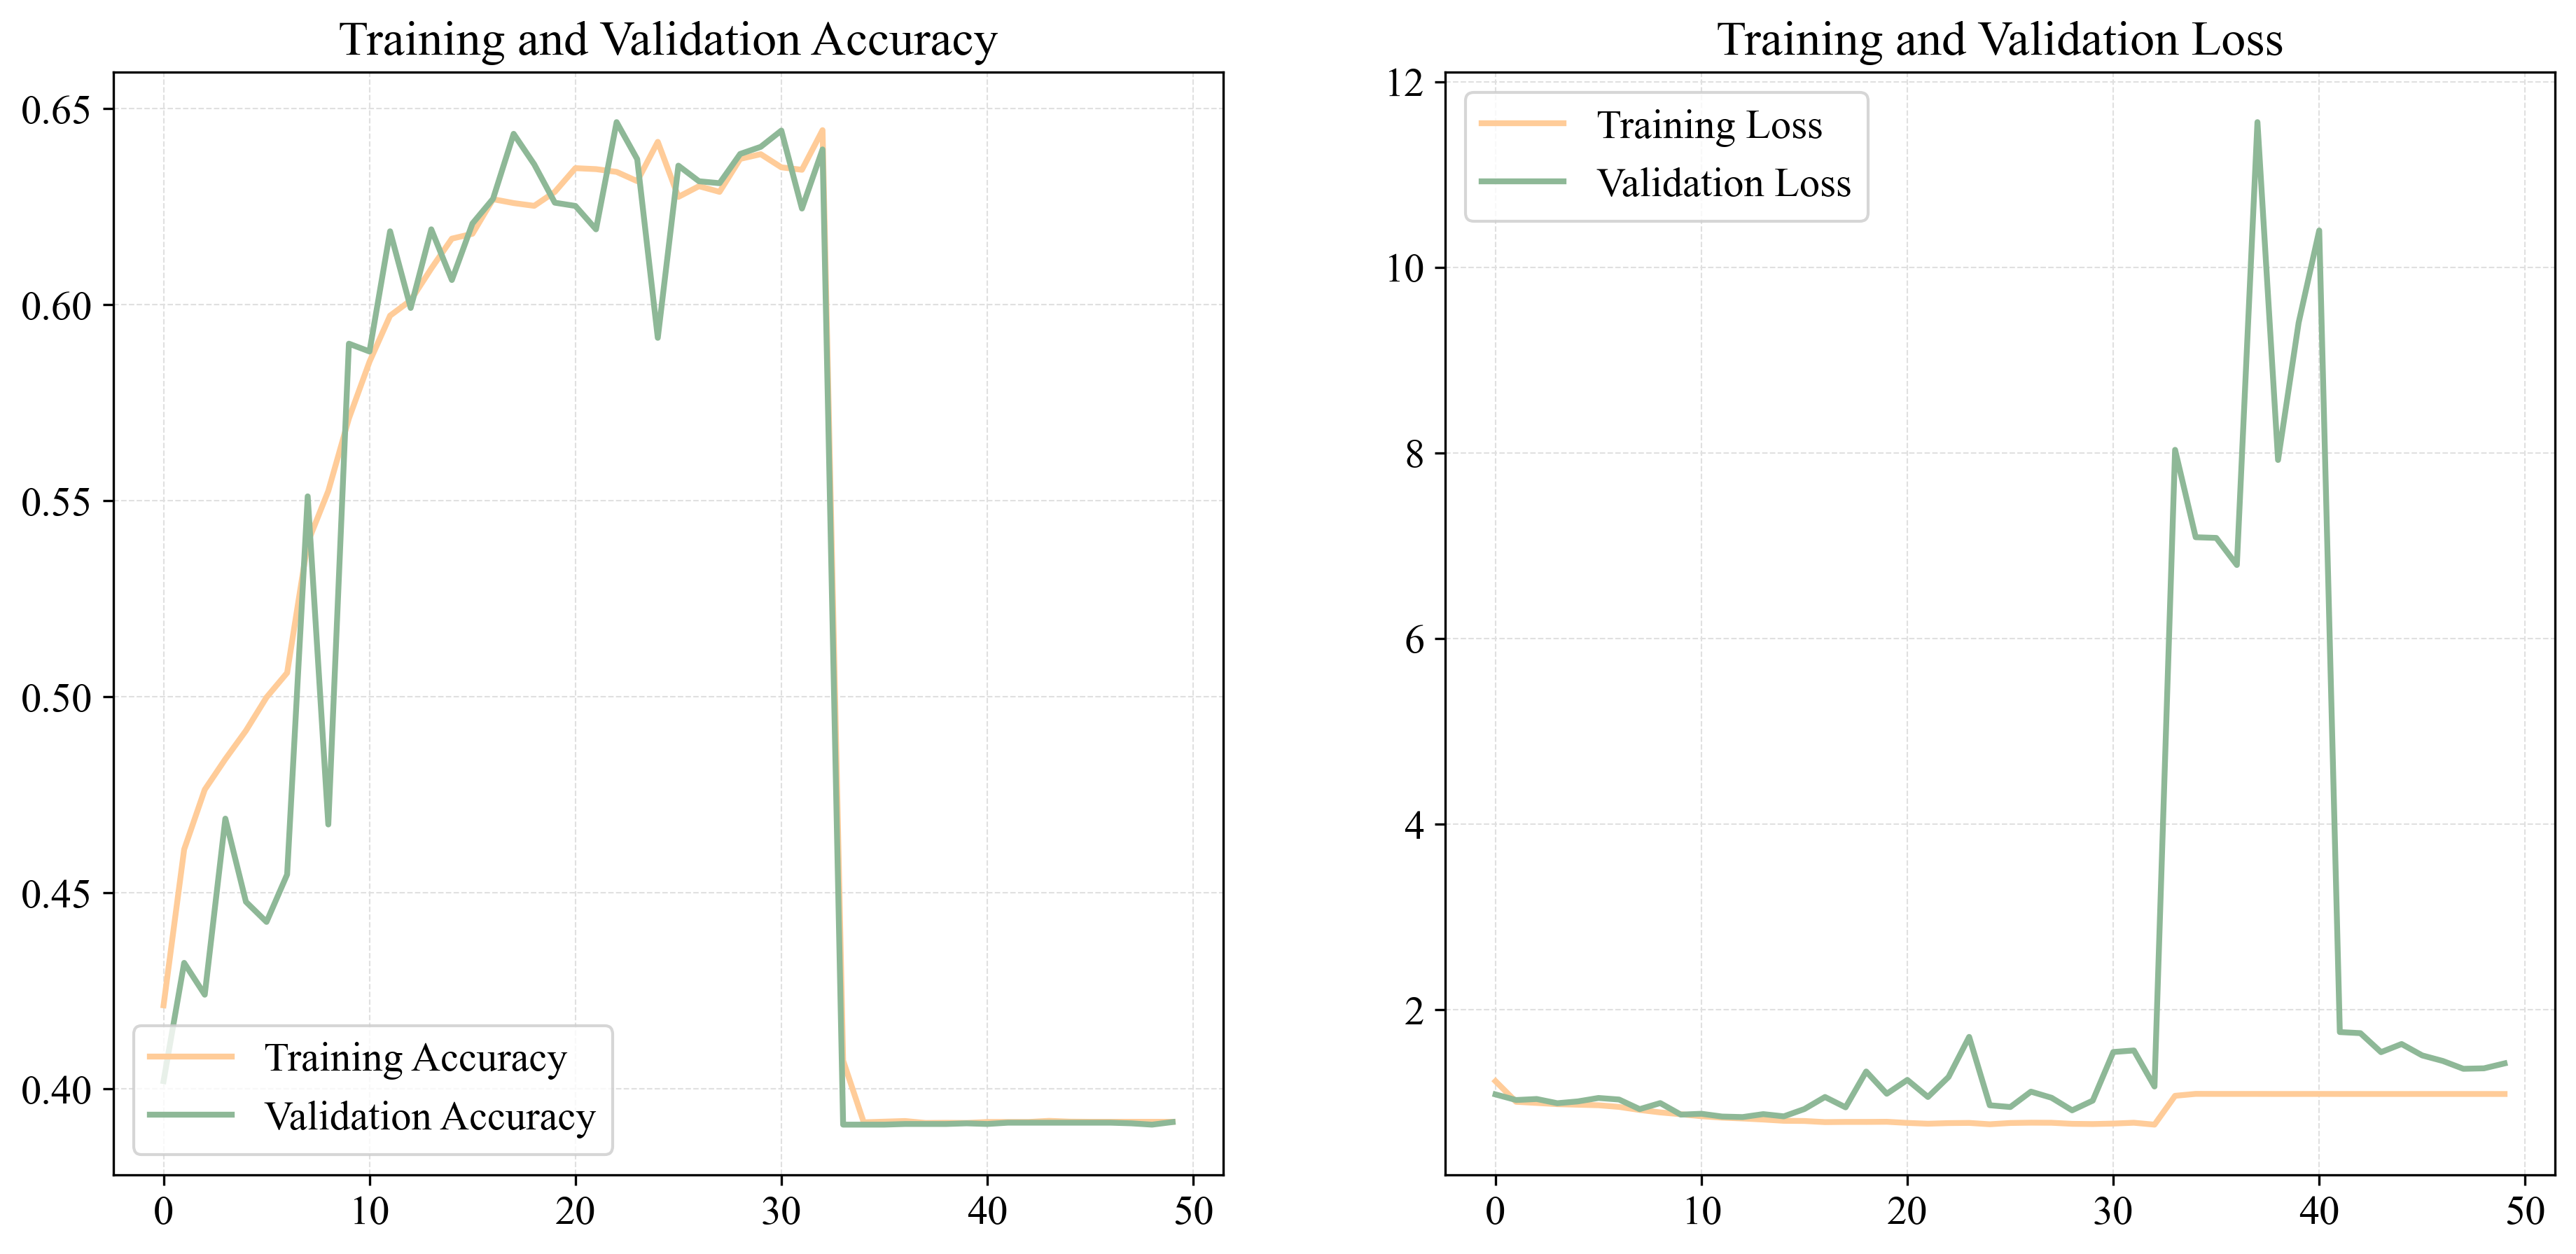
\includegraphics[width=0.8\textwidth]{figures/Figure30.png}
    \caption{Training and Validation Accuracy and Loss Curves for Model 2}
    \label{fig:chap3 figure2}
\end{figure}


\textbf{Key Observations:}
\begin{itemize}
    \item \textbf{Training Accuracy and Loss:} The training accuracy for Model 2 shows an improvement over Model 1, indicating better learning of the patterns in the training data. The training loss also decreases steadily, demonstrating effective optimization.
    \item \textbf{Validation Accuracy and Loss:} The validation accuracy for Model 2 is more stable compared to Model 1, suggesting improved generalization. However, the validation loss still shows fluctuations, indicating that further adjustments might be necessary to achieve optimal performance.
\end{itemize}

The results suggest that Model 2, with the Adam optimizer, provides a more stable learning process and better generalization compared to Model 1. Nonetheless, continued experimentation with different architectures and hyperparameters will be crucial to further enhance the model's performance on the validation set.

The model building for classification based on class labels is concluded at this juncture. The results obtained from the current CNN architectures indicate that while there is potential for improvement, further refinements are necessary to achieve optimal performance. Consequently, the focus will now shift to developing models for predicting the target variable, which signifies the presence or absence of pneumonia. For the classification task based on class labels, additional fine-tuning and enhancements will be undertaken using Region-based Convolutional Neural Networks (RCNN) during phase 2 of the project. This phased approach ensures that the models are progressively improved, leveraging advanced techniques to enhance their accuracy and reliability in detecting pneumonia.

Model 3 was designed with a simplified architecture compared to Models 1 and 2. It consists of:
\begin{itemize}
    \item Two convolutional blocks, each followed by max pooling and dropout layers, to reduce overfitting.
    \item A global max pooling layer to reduce the dimensionality of the feature maps.
    \item A dense layer with 128 units and ReLU activation, followed by a dropout layer to further prevent overfitting.
    \item An output layer with a softmax activation function for multi-class classification.
\end{itemize}
Figure \ref{fig:chap3 figure3} shows the training and validation accuracy and loss curves for Model 3.

\begin{figure}[H]
    \centering
    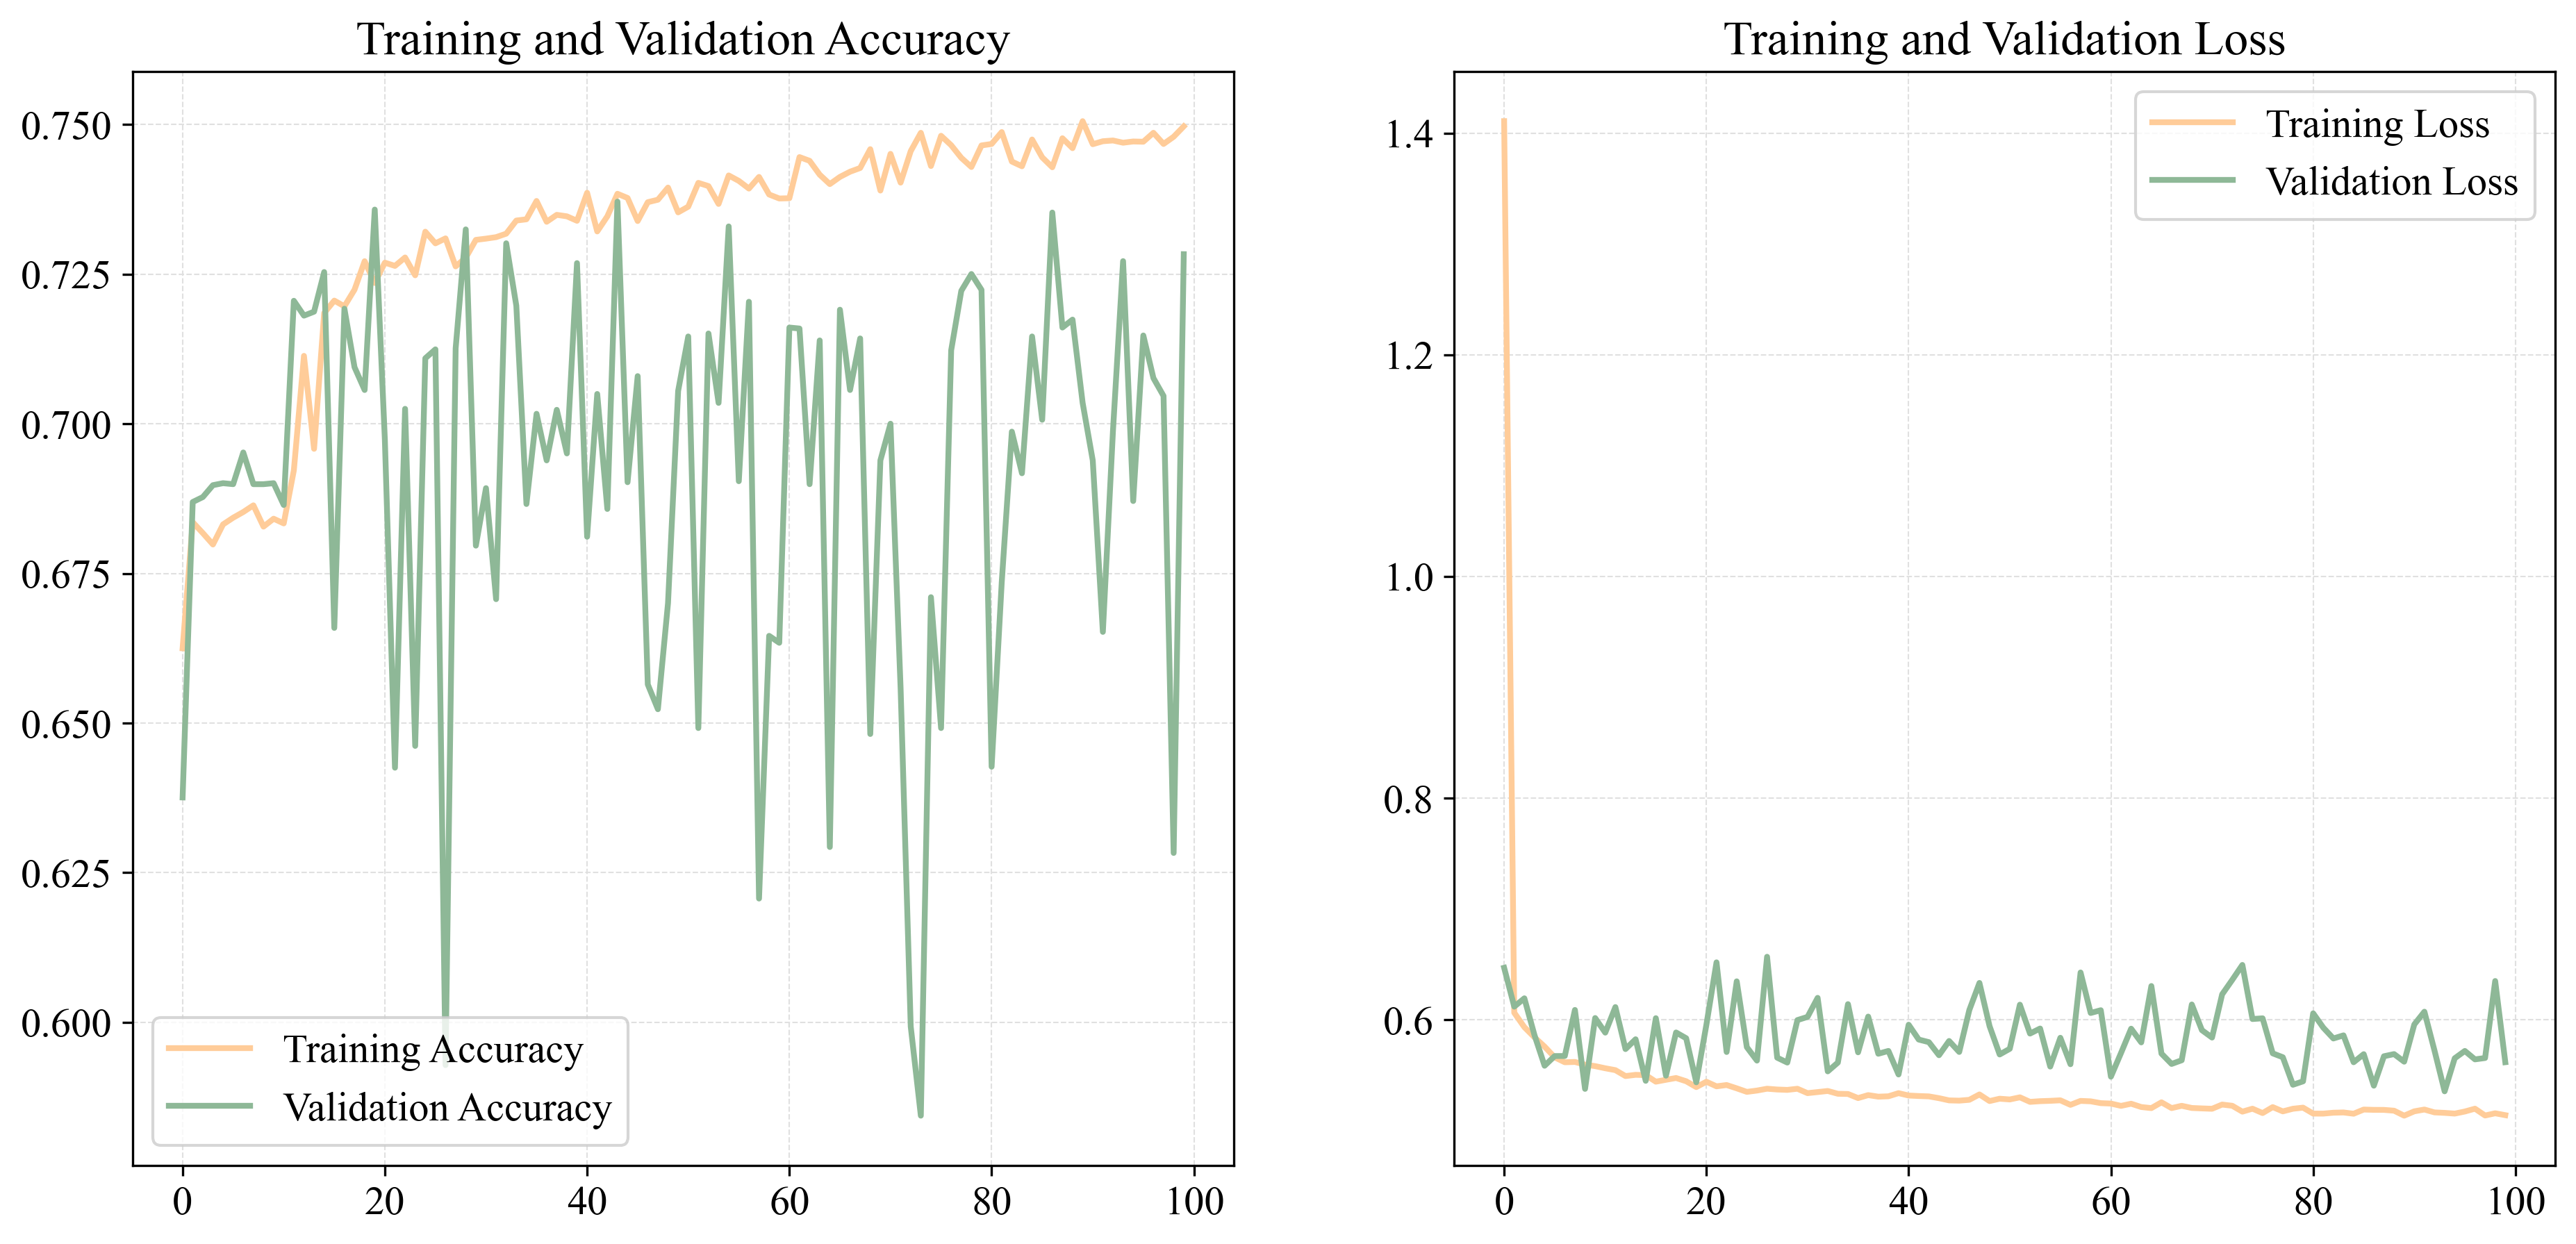
\includegraphics[width=0.8\textwidth]{figures/Figure31.png}
    \caption{Training and Validation Accuracy and Loss Curves for Model 3}
    \label{fig:chap3 figure3}
\end{figure}

\textbf{Key Observations:}
\begin{itemize}
    \item The training and validation accuracy curves indicate that Model 3 achieved better stability compared to Models 1 and 2.
    \item The training accuracy started around 0.60 and steadily increased, stabilizing around 0.75 towards the end of the training.
    \item The validation accuracy also showed a steady improvement, with minor fluctuations, reaching approximately 0.70.
    \item The training and validation loss curves suggest that the model is learning effectively with no major signs of overfitting or underfitting.
    \item Despite the fluctuations, the validation accuracy consistently stayed close to the training accuracy, indicating good generalization.
\end{itemize}

Model 3 demonstrated improved stability and generalization compared to the previous models. Its simplified architecture, combined with effective dropout and pooling strategies, contributed to achieving better performance metrics. The consistent validation accuracy suggests that Model 3 is a suitable candidate for further fine-tuning and optimization, particularly for predicting the target variable indicating the presence of pneumonia.